\documentclass{article}

\usepackage{amsmath}
\usepackage{graphicx}
\usepackage{hyperref}
\usepackage{tabularx}
\usepackage{xcolor}
\usepackage{float}


\title{Note on Tree of Thoughts: Deliberate Problem Solving with Large Language Models}

\begin{document}


\maketitle

\section{Motivation}

\textbf{Shortcoming} of current paradigm-original autoregressive mechanisms: Current LLMs 
fall short in tasks that require exploration, strategic lookahead, or where initial decisions 
play a pivotal role.

\begin{itemize}
    \item Locally, they do not explore different continuations within a thought process – the branches of the tree.
    \item Globally, they do not incorporate any type of planning, lookahead, or backtracking to help evaluate these different options – the kind of heuristic-guided search that seems characteristic of human problem-solving.
\end{itemize}

Analogous to the two modes of human thought, the simple associative token-level choices of 
LMs are reminiscent of "System 1"- a fast, automatic, unconscious mode. Thus might benefit from 
augmentation by a more delibrate "System 2" which can 

\begin{itemize}
    \item maintains and explores diverse alternatives for current choices instead of just picking one
    \item evaluates its current status and actively looks ahead or backtracks to make more global decisions
\end{itemize}

This paper the \textbf{Tree of Thoughts} (TOT) framework for general problem solving with LMs.

\begin{figure}[H]
    \centering
    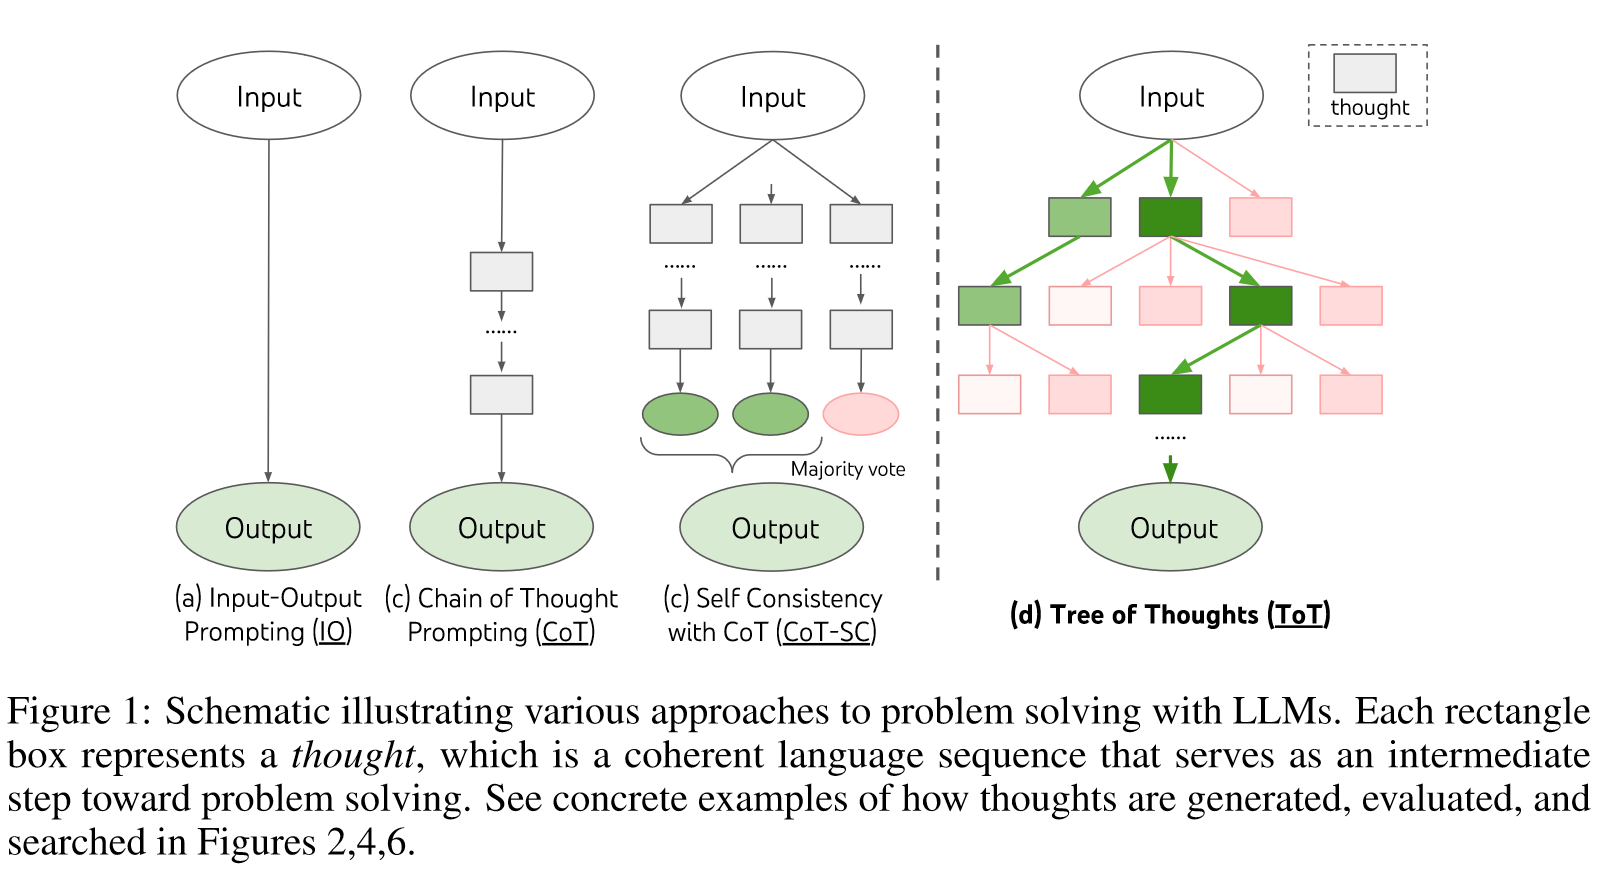
\includegraphics[width=\textwidth]{./Images/Figure1.png}
    \caption{Schematic illustrating various approaches to problem solving with LLMs. Each rectangle box represents a thought, which is a coherent language sequence that serves as an intermediate step toward problem solving.}
    \label{fig:Figure1}
\end{figure}

As Figure \ref{fig:Figure1} illustrates, while existing methods (detailed below) sample continuous language sequences for problem solving, ToT actively maintains a tree of thoughts, where each thought is a coherent language sequence that serves as an intermediate step toward problem solving (Table \ref{tab:Table1})

Finally, This paper combine this language-based capability to generate and evaluate diverse thoughts with search algorithms, such as breadth-first search (BFS) or depth-first search (DFS), which allow systematic exploration of the tree of thoughts with lookahead and backtracking.


\section{Background}

Formalize existing methods that use large language models for problem-solving, which ToT is inspired 
by and later compared with. $p_{\theta}$ denote a pre-trained LM with parameters $\theta$, and 
\textbf{lowercase letters} \textit{x,y,z,s, ...} denote a langauage sequence, i.e.x = (x[1],...,x[n])
 where each x[i] is a token, so that $p_{\theta}(x) = \prod_{i=1}^{n}p_{\theta}(x[i]|x[1...i])$. Use uppercase 
 S, ... to denote a collection of language sequences.

\begin{itemize}
    \item \textbf{Input-output (IO) prompting}: turn a problem input x into output y with LM: $y\sim p_{\theta}(y|prompt_{IO}(x)),
    $ where $prompt_{IO}(x)$ wraps input x with task instructions and/or few-shot input-output examples. For simplicity, denote $p^{prompt}_{\theta}(output|input)=p_{\theta}(output|prompt(input))$,
     so that IO prompting can be formulated as $y \sim p_{\theta}^{IO}{y|x}$.
    \item \textbf{Chain-of-thought (CoT) prompting}: proposed to address cases where the mapping of input x to output y is non-trivial (e.g. when x is a math question and y is the final numerical answer).
    introduce a chain of \textit{thoughts} $z_1, ... , z_n$ to bridge x and y, where each $z_i$ is a coherent language sequence that serves as a meaningful intermediate step toward problem solving. (e.g. $z_i$ could be an intermediate equation for math QA).
    To solve problems with CoT, each thought $z_i \sim p^{CoT}_{\theta}(z_i | x, z_{1...i-1})$ is sampled sequentially, then the output $y \sim p^{CoT}_{\theta}(y|x,z_{1...n})$. In practice, $[z_{1...n},y] \sim p^{CoT}_{\theta}(z_{1...n},y | x)$ 
    is sampled as a continuous language sequence, and the \textbf{decomposition} of thoughts (e.g. is each $z_i$ a phrase, a sentence, or a paragraph) is left ambiguous.
    \item \textbf{Self-consistency with CoT (CoT-SC)}: an ensemble approach that samples k i.i.d chains of thought: 
    $[z_{1...n}^{(i)},y^{(i)}]\sim p^{CoT}_{\theta}(z_{1...n},y|x)(i=1...k)$, then returns the most frequent output: $\textit{arg max}_y \# {i|y^{(i)}=y}.$

\end{itemize}

\section{Tree of Thoughts: Deliberate Problem Solving with LM}

\textbf{Tree of Thoughts:} a paradigm that allows LMs to explore multiple reasoning paths over thoughts(Figure (\ref{fig:Figure1})(c))
ToT frames any problem as a search over a tree, where each node is a \textbf{state} $s = [x,z_{1...i}]$ representing a partial solution with the input and the sequence of thoughts so far.

\subsection*{1.Thought decomposition}
As Table \ref{tab:Table1} shows, depending on different problems, a thought could be a couple of words (Crosswords), a line of equation (Game of 24), or a whole paragraph of writing plan (Creative Writing).
In general, a thought should be “small” enough so that LMs can generate promising and diverse samples (e.g. generating a whole book is usually too “big” to be coherent), yet “big” enough so that LMs can evaluate its prospect toward problem solving (e.g. generating one token is usually too “small” to evaluate).

\subsection*{2.Thought generator $G(p_{\theta},s,k)$}
Given a tree state $s = [x,z_1...i]$, this paper consider two strategies to generate k candidates for the next thought step:
\begin{itemize}
    \item \textbf{Sample} i.i.d thoughts from a CoT prompt (Creative Writing, Figure \ref{fig:Figure4}): $z^{(j)} \sim p^{CoT}_{\theta}(z_{i+1}|s) = p^{CoT}_{\theta}(z_{i+1}|x,z_{1...i})(j=1...k)$.
    \item \textbf{Propose} thoughts sequentially using a “propose prompt” (Game of 24, Figure \ref{fig:Figure2}; Crosswords, Figure \ref{fig:Figure6}: 
    $[z^{(1)},...,z^{(k)}]\sim p^{propose}_{\theta}(z^{(1...k)_(i+1)}|s)$).
    \item \textbf{State evaluator $V(p_{\theta},S)$}. using the LM to deliberately reason about states. consider two strategies to evaluate states either independently or together:
        \subitem \textbf{Value} each state independently: $V(p_{\theta},S)(s) \sim p^{value}_{\theta}(v|s) \forall s \in S$, where a value prompt reasons about the state s to generate a scalar value v
            or a classification (e.g. sure/likely/impossible) that could be heuristically turned into a value.
        \subitem \textbf{Vote} across states: $V(p_{\theta},S) = 1 [s = s^{*}]$, where a “good” state $s^* \sim p_{\theta}^{vote}(s^*|S)$ is voted out based on deliberately comparing different states in S in a vote prompt.
    \item \textbf{Search algorithm.} BFS and DFS
\end{itemize}

\begin{table}[H]
    \centering
    \begin{tabularx}{\textwidth}{|X|X|X|X|}
        \hline
        & \textbf{Game of 24} & \textbf{Creative Writing} & \textbf{5 $\times$ 5 Crosswords} \\
        \hline
        \textbf{Input} & 4 numbers \textcolor{blue}{(4 9 10 13)} & 4 random sentences & 10 clues \textcolor{blue}{(h1. presented;..)}\\
        \hline
        \textbf{Output} & An equation to reach 24\textcolor{blue}{(13-9)*(10-4)=24} & A passage of 4 paragraphs ending in the 4 sentences & 5x5 letters: \textcolor{blue}{SHOWN; WIRRA; AVAIL; ...} \\
        \hline
        \textbf{Thoughts} & 3 intermediate equations \textcolor{blue}{(13-9=4 (left 4,4,10); 10-4=6 (left 4,6); 4*6=24)} & A short writing plan \textcolor{blue}{(1. Introduce a book that connects...)} & Words to fill in for clues: \textcolor{blue}{(h1. shown; v5. naled; ...)} \\
        \hline
        \textbf{\#ToT steps} & 3 & 1 & 5-10 (variable) \\
        \hline
        \end{tabularx}

        \caption{Task overview. Input, output, thought examples are in blue}
        \label{tab:Table1}
\end{table}

\begin{figure}[H]
    \centering
    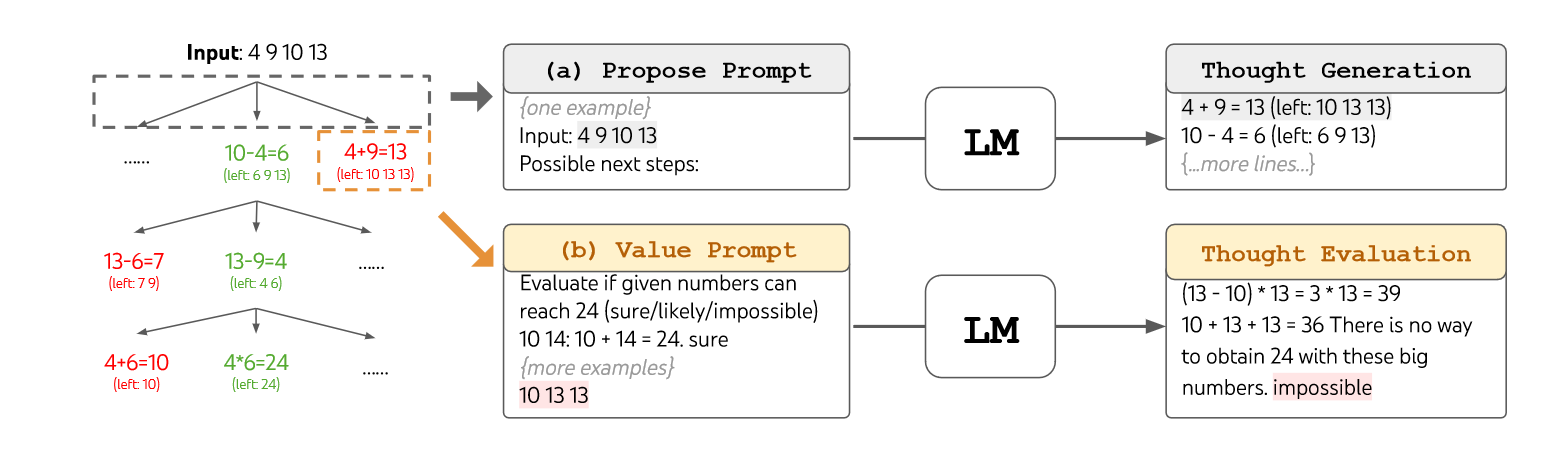
\includegraphics[width=\textwidth]{./Images/Figure2.png}
    \caption{ToT in a game of 24. The LM is prompted for (a) thought generation and (b) valuation.}
    \label{fig:Figure2}
\end{figure}

\begin{figure}[H]
    \centering
    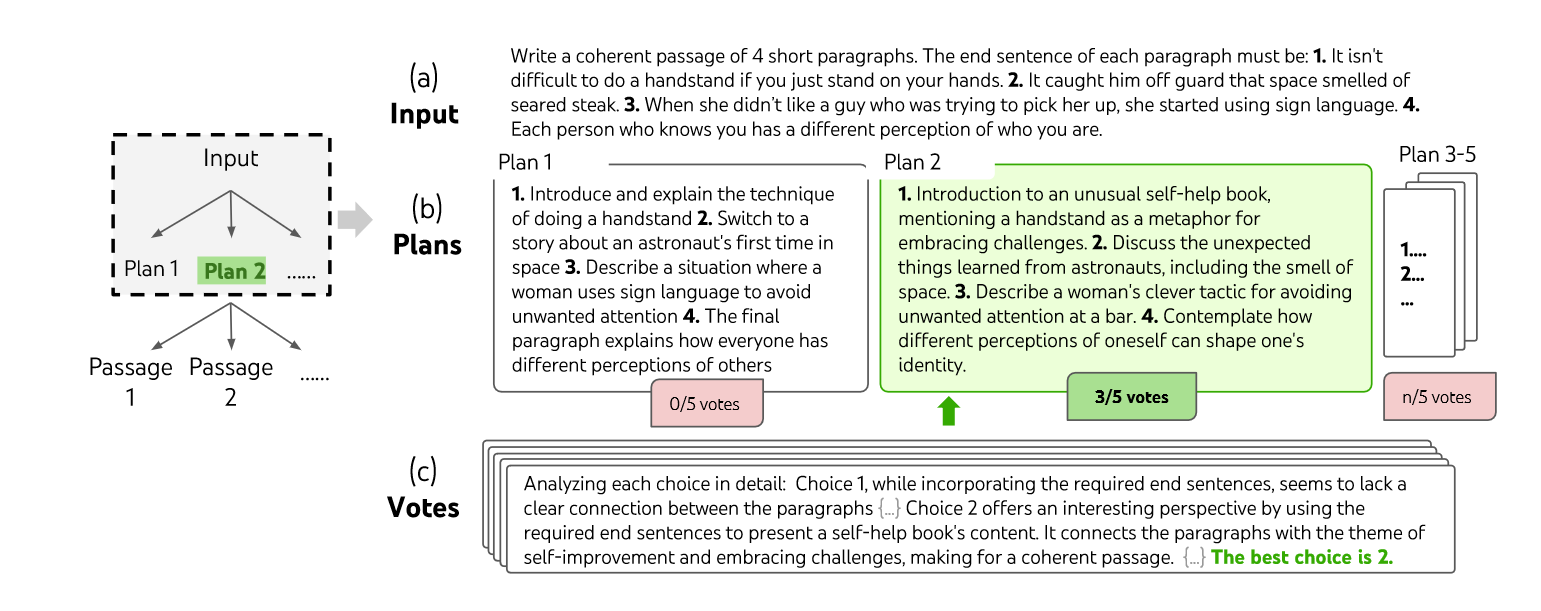
\includegraphics[width=\textwidth]{./Images/Figure4.png}
    \caption{A step of deliberate search in a randomly picked Creative Writing task. Given the input, the LM samples 5 different plans, then votes 5 times to decide which plan is best. The majority choice is used to consequently write the output passage with the same sample-vote procedure.}
    \label{fig:Figure4}
\end{figure}

\begin{figure}[H]
    \centering
    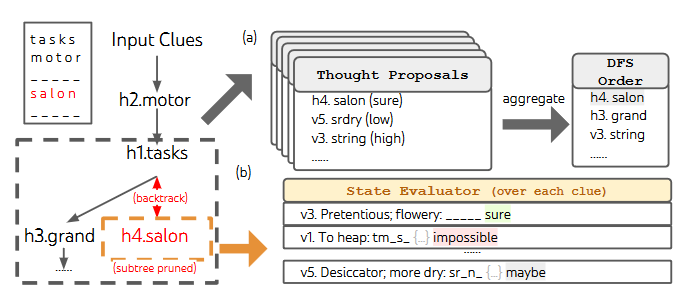
\includegraphics[width=\textwidth]{./Images/Figure6.png}
    \caption{In Mini Crosswords, (a) how thoughts are proposed and aggregated in a priority queue for depth-first search (DFS), and (b) how a state is evaluated based on the possibility of filling in each remaining word clue, and pruned if any remaining clue is deemed not possible to fill by the LM. Then DFS backtracks to the parent state and explore the next promising thought for clue.}
    \label{fig:Figure6}
\end{figure}

\end{document}